% !TeX root = ../main.tex
% !TEX spellcheck = en_GB

\chapter{Design}
\label{ch:Design}

\section{Overall}
\section{Sequence Diagrams}
The sequence diagrams (SD) below are meant to give an understanding of the inner workings of the \systemName.

Initiation of the system is described in \cref{fig:SD:init}.
It shows the µC initiating itself and then the external blocks.
The GPS module is polled until it returns valid location data. The time returned from the GPS allows the µC know the time and run the desired actions either at certain intervals, e.g. every 10 minutes, or at specific times, e.g. every full hour.
When valid data has been retrieved it is saved to the SD card and the GPS and GSM modules are put to sleep to conserve power.
The acquisition of GPS location is shown in \cref{fig:SD:getlocation}.
The GPS starts in a sleep mode and is awoken to find it's location.
When the location is found and is valid, the GPS is put back to sleep and the data is saved tot he SD card.
To upload data to the server, the GSM must be awoken and data must be retrieved from the SD card, as shown in \cref{fig:SD:upload}.
When the data has been sent the GSM is put back to sleep.

\begin{figure}
	\centering
	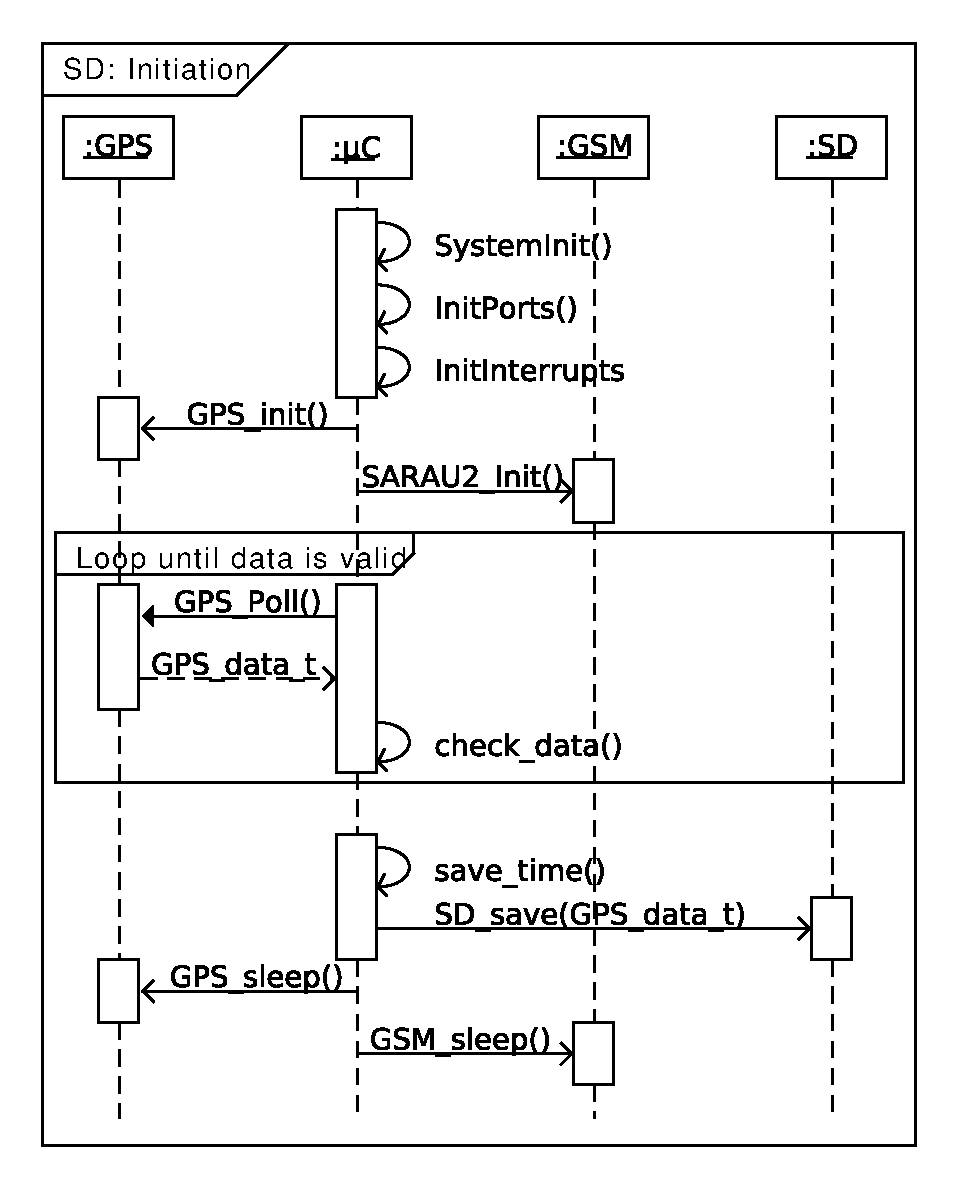
\includegraphics[width=0.7\linewidth]{gfx/Design/SD_init.pdf}
	\caption{Sequence diagram showing the initiation of the system.}
	\label{fig:SD:init}
\end{figure}

\begin{figure}
	\centering
	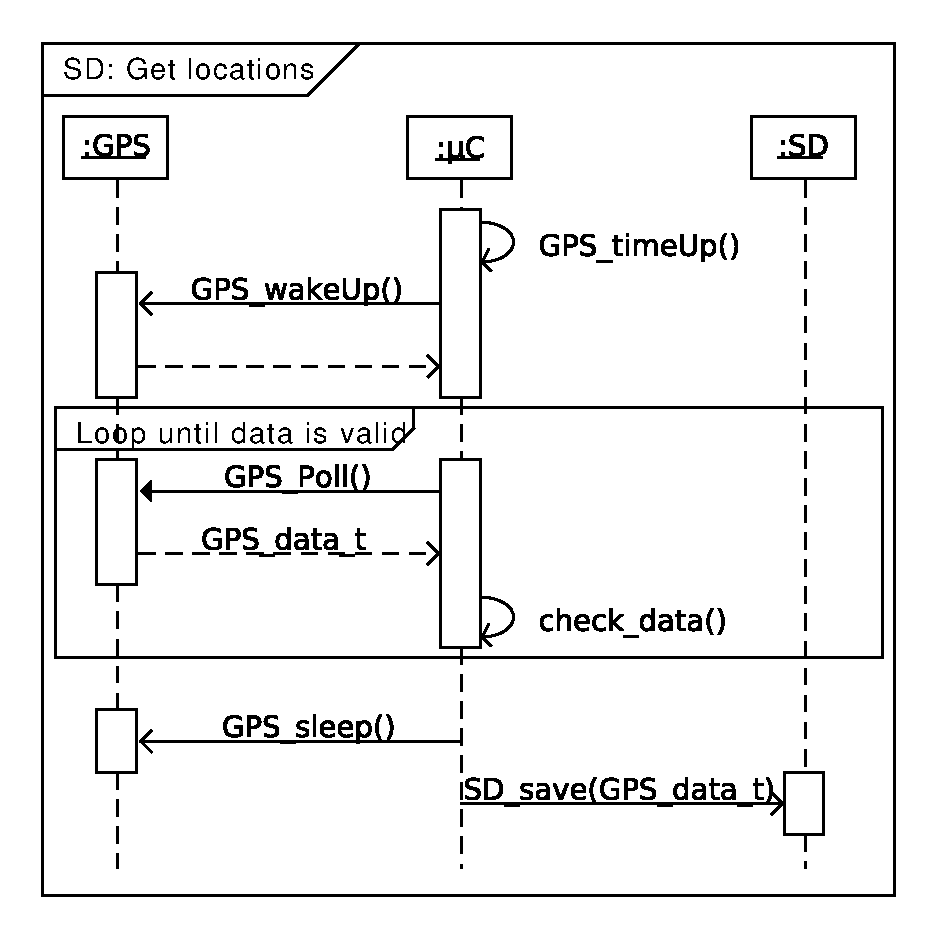
\includegraphics[width=0.7\linewidth]{gfx/Design/SD_getLocation.pdf}
	\caption{Sequence diagram describing the acquisition and saving of GPS data.}
	\label{fig:SD:getlocation}
\end{figure}

\begin{figure}
	\centering
	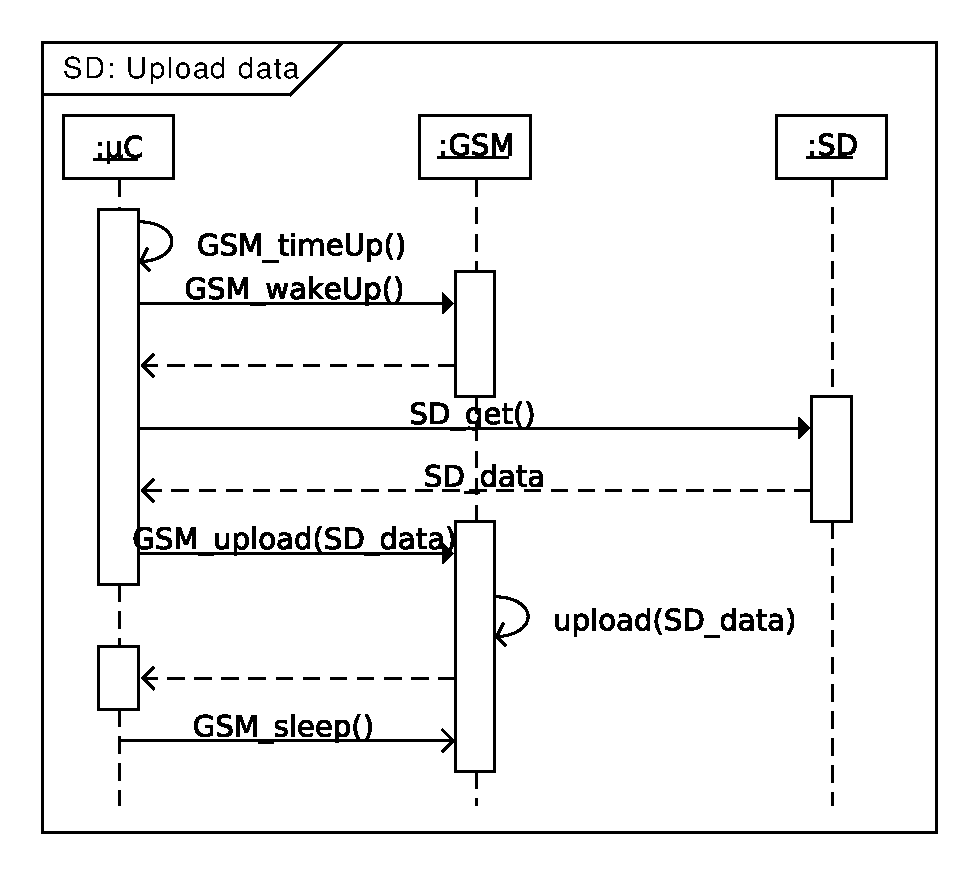
\includegraphics[width=0.7\linewidth]{gfx/Design/SD_Upload.pdf}
	\caption{Sequence diagram showing the process of sending saved data to the server.}
	\label{fig:SD:upload}
\end{figure}

\section{GSM - \SARA}
To facilitate the functionality of the \SARA module, a modem specific driver will be developed. This driver will contain functions to configure \SARA for sending and receiving data through UDP packets.
\fxnote{State diagram?}

\subsection{UART}
Communication with the \SARA module, will be done through a UART connection. The module contains an ability to auto detect the baud rate of the first transmission, and use this baud rate to respond. In addition it supports the standard baud rates: \num{1200}, \num{2400}, \num{4800}, \num{9600}, \num{19200}, \num{38400} and 5 higher rates. \num{9600} baud was selected with focus on stability and the ability to debug the communications.

\subsection{AT Command Interface}
\fxnote{Describe - Sequence of AT commands}
As is standard with GSM modules, the \SARA employs a AT command interface through the UART. This means that commands and data to and from the module is in ascii, and that commands is started by "+AT" and end with <CR><LF>. In this application a limited amount of commands is necessary, the flow and functionality is display on \fxnote{FIGUR Ref}. The commands used are described, in appendix table. \fxnote{Insert GSMSetupConnection.pdf and ref to Appendix}

\section{GPS - \GPS}




\fxnote{Choices + Diagrammer}

\section{SD-card - \SDsock}


\section{UART - \SAMD}



\subsection{BaudRate}
Both \SARA and \GPS supports the usage of auto baud rate detection, meaning that they will respond to a message in the same baud rate as they receive.
But due to consistency, both modules is set to the selected baud rate during their set up configuration. 
For simplicity a baud rate of \SI[per-mode = symbol]{9600}{\bit\per\second} was chosen, specification for the UART is shown in \vref{tab:BaudRate}.

\begin{table}[H]
	\begin{tabular}{ll}
		\hline 
		Baud Rate & 9600 \\ 
		\hline 
		Data Bits & 8 \\ 
		\hline 
		Parity & None \\ 
		\hline 
		Stop Bits & 1 \\ 
		\hline 
	\end{tabular}
	\centering
	\caption{Baud rate definition used for serial com ports on \SAMD.}
	\label{tab:BaudRate}
\end{table} 

\FloatBarrier